\section{Wyniki Eksperymentów}

Dla każdej architektury przeprowadzono grid search z 5-fold cross-validation.

\subsection{Porównanie architektur}

\begin{figure}[H]
\centering
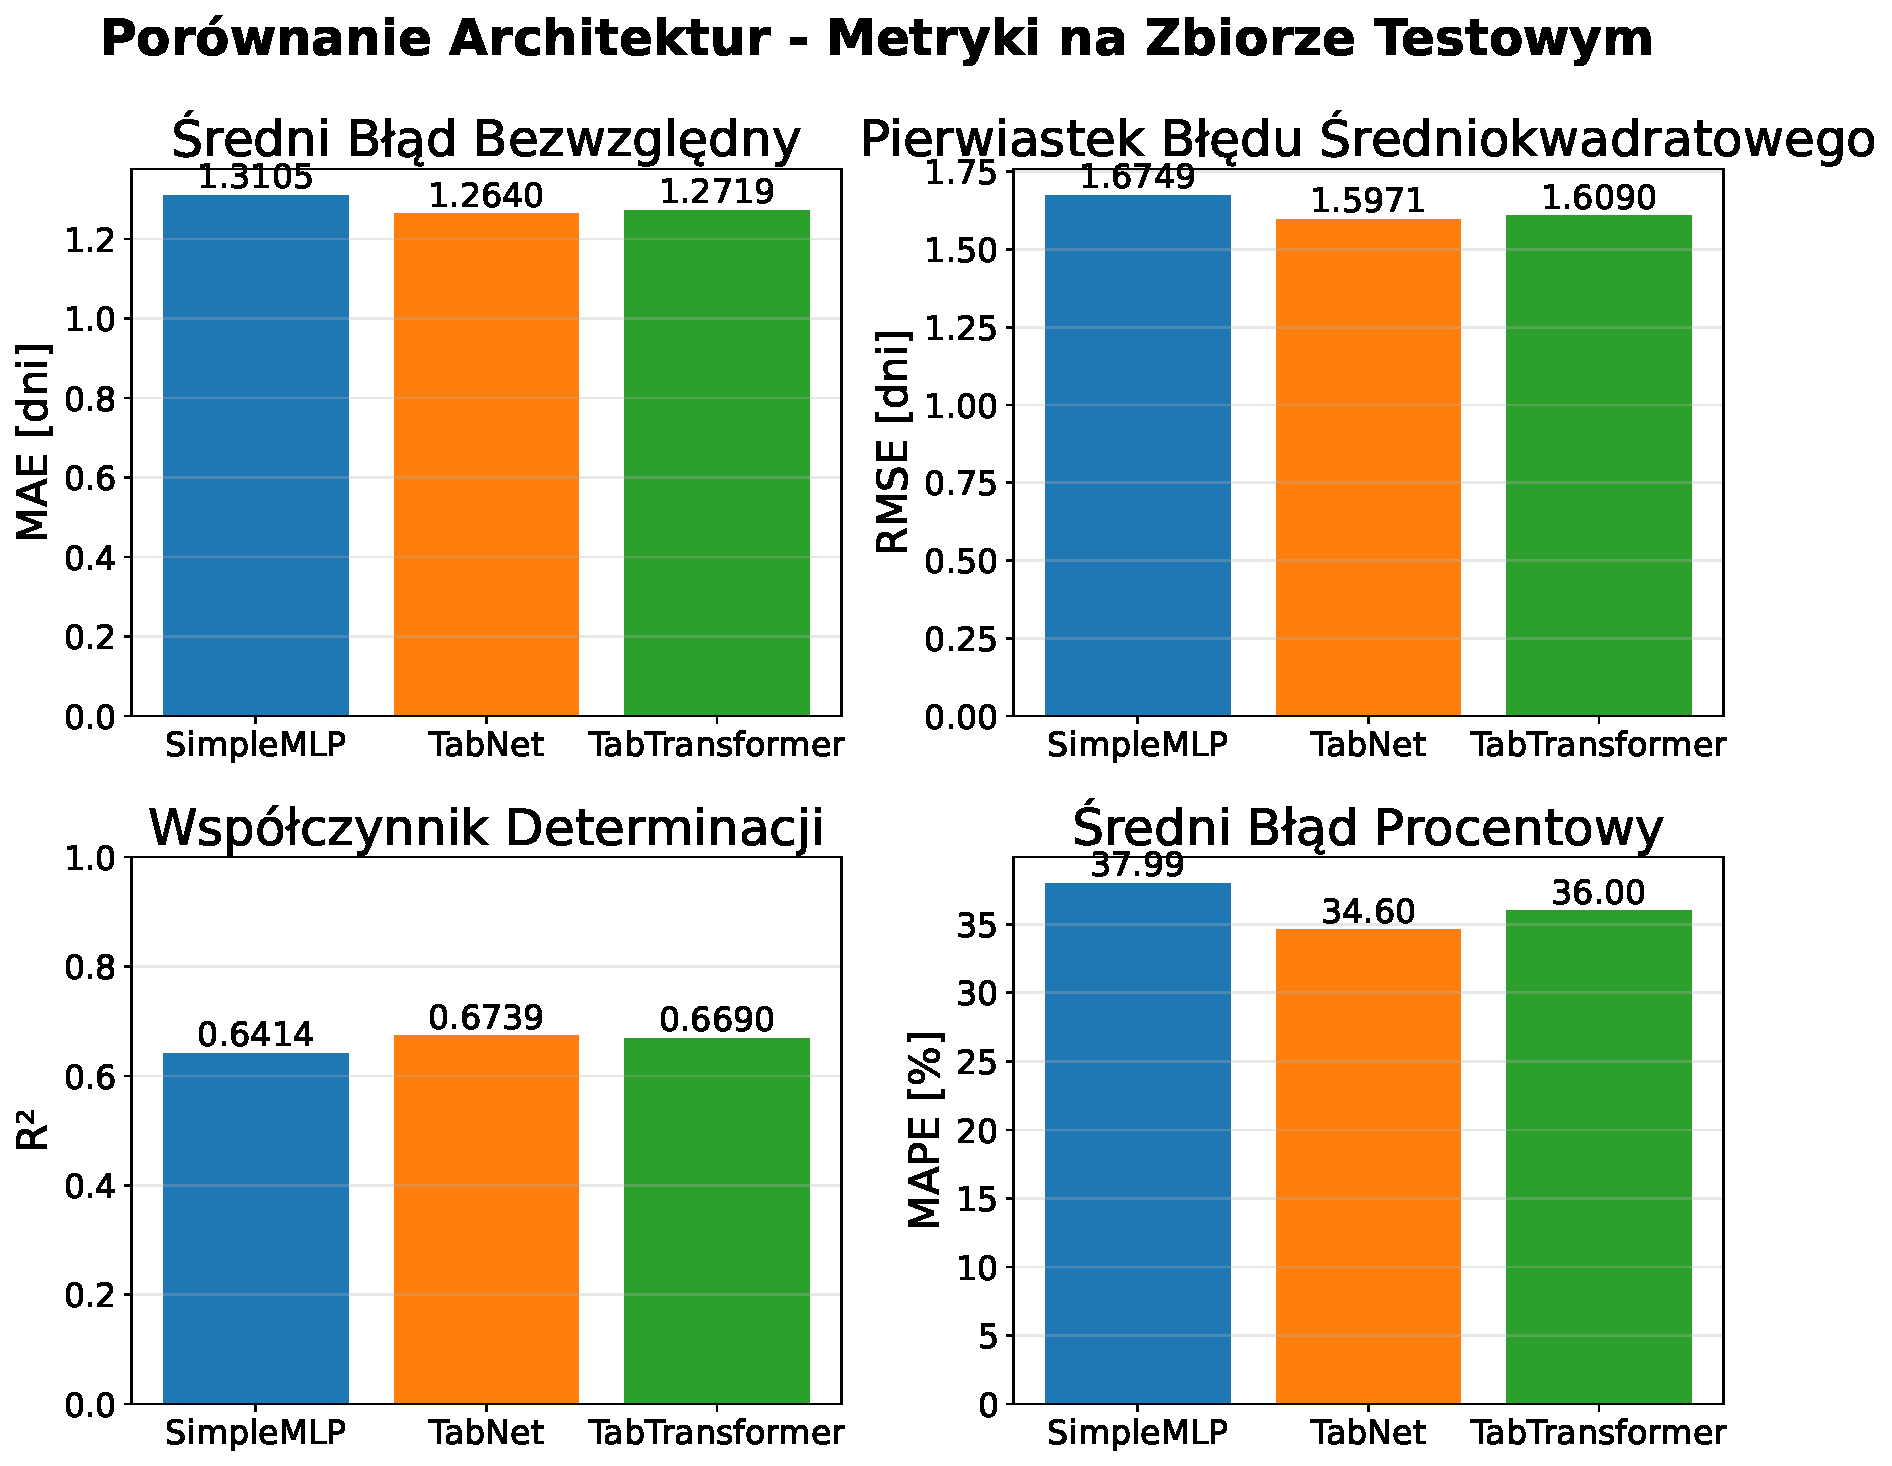
\includegraphics[width=0.95\textwidth]{figures/architecture_comparison.pdf}
\caption{Porównanie architektur - metryki testowe}
\end{figure}

\begin{figure}[H]
\centering
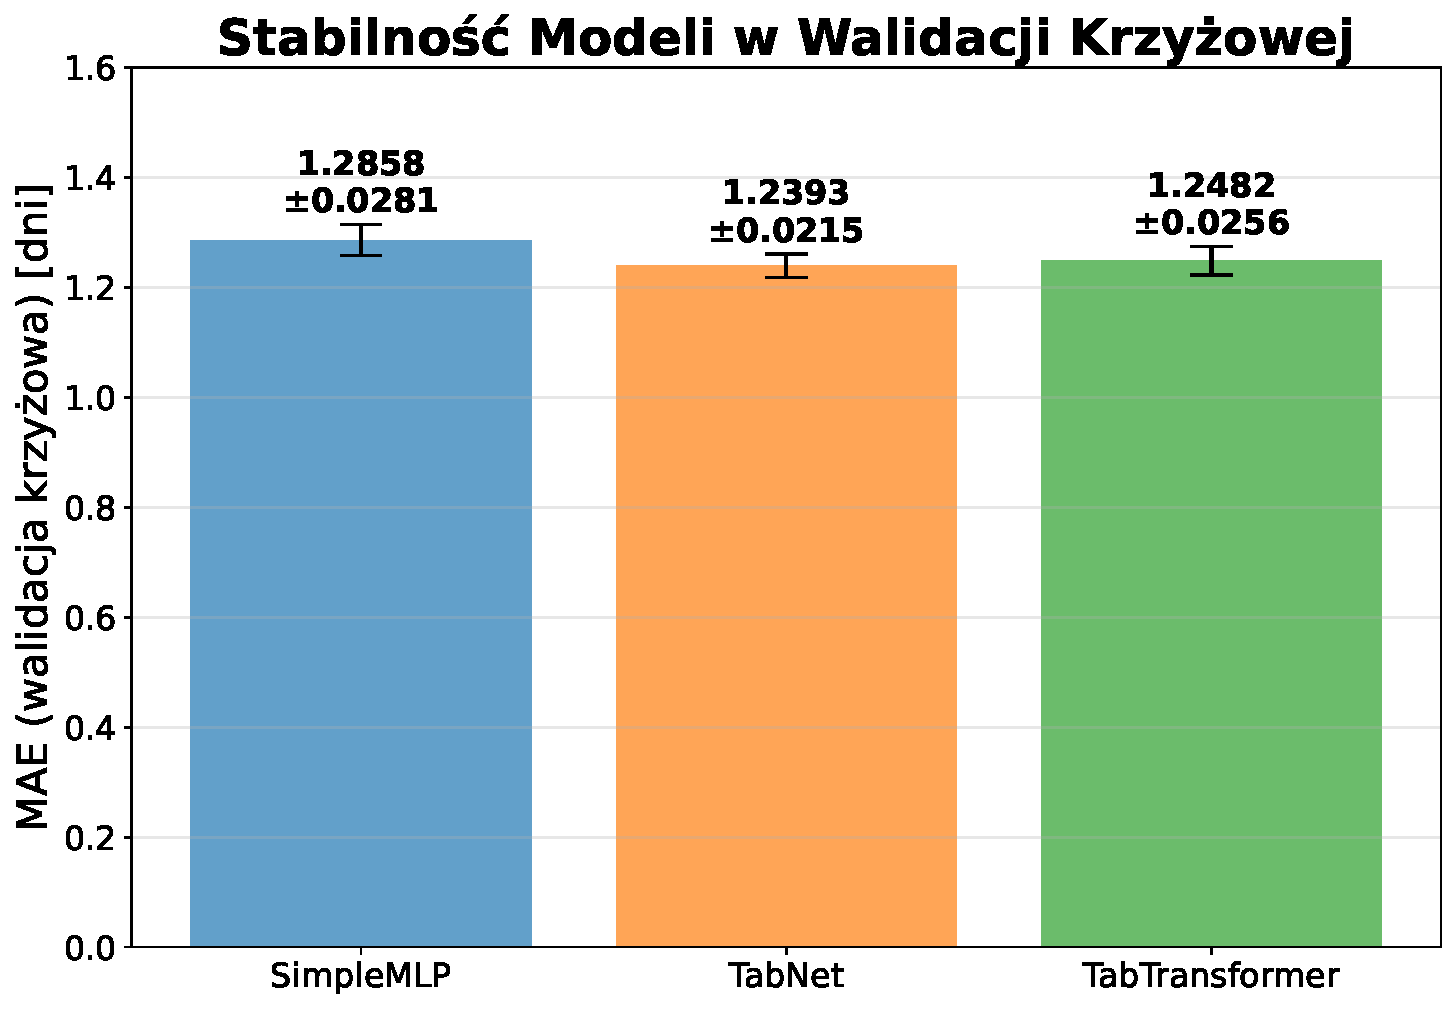
\includegraphics[width=0.75\textwidth]{figures/cv_stability.pdf}
\caption{Stabilność modeli w walidacji krzyżowej}
\end{figure}

TabNet osiągnął najlepsze wyniki we wszystkich metrykach.

\subsection{SimpleMLP}

\begin{table}[H]
\centering
\caption{Najlepszy model SimpleMLP}
\begin{tabular}{lc}
\toprule
Parametr & Wartość \\
\midrule
Hidden features & 256 \\
Dropout & 0.2 \\
Activation & ReLU \\
MAE (CV) & 1.2858 $\pm$ 0.0281 \\
MAE (Test) & 1.3105 \\
R² (Test) & 0.6414 \\
\bottomrule
\end{tabular}
\end{table}

\subsection{TabNet}

\begin{table}[H]
\centering
\caption{Najlepszy model TabNet}
\begin{tabular}{lc}
\toprule
Parametr & Wartość \\
\midrule
n\_d & 64 \\
n\_a & 32 \\
n\_steps & 3 \\
MAE (CV) & 1.2393 $\pm$ 0.0215 \\
MAE (Test) & \textbf{1.2640} \\
R² (Test) & \textbf{0.6739} \\
\bottomrule
\end{tabular}
\end{table}

\subsection{TabTransformer}

\begin{table}[H]
\centering
\caption{Najlepszy model TabTransformer}
\begin{tabular}{lc}
\toprule
Parametr & Wartość \\
\midrule
d\_model & 128 \\
n\_heads & 2 \\
num\_layers & 2 \\
MAE (CV) & 1.2482 $\pm$ 0.0256 \\
MAE (Test) & 1.2719 \\
R² (Test) & 0.6690 \\
\bottomrule
\end{tabular}
\end{table}
